\documentclass[aspectratio=169,11pt]{beamer}
\usepackage[utf8]{inputenc}
\usepackage[T1]{fontenc}
\usepackage{booktabs,amsmath,amssymb}
\usepackage{tikz}
\usetikzlibrary{arrows.meta,positioning,shapes.geometric,calc}
\usetheme{default}
\usecolortheme{seahorse}
\setbeamertemplate{navigation symbols}{}
\setbeamertemplate{footline}{\hfill\insertframenumber/\inserttotalframenumber\hspace{2mm}\vspace{2mm}}
\definecolor{vw}{RGB}{0,30,80}
\setbeamercolor{frametitle}{bg=vw,fg=white}
\setbeamercolor{title}{bg=vw,fg=white}
\setbeamerfont{frametitle}{size=\large,series=\bfseries}

\tikzset{
  box/.style={draw,rounded corners=2pt,align=center,font=\small,inner sep=4pt,minimum height=7mm,fill=gray!8},
  kg/.style={box,fill=blue!10}, db/.style={box,fill=orange!15}, app/.style={box,fill=green!10},
  arr/.style={-{Stealth[length=2mm]},thick},
  lbl/.style={font=\scriptsize,fill=white,inner sep=1pt}
}

\title{Hybrid Knowledge Graph + SQL Expert System\\for Automotive Cost, Contract and Strategy Analysis}
\author{Anjar Tiyo Saputro \and Edgar Puyou-Bracq}
\institute{Artificial Intelligence Principles\\Department of Computer Science and Electronics\\Universitas Gadjah Mada}
\date{\today}

\begin{document}

\begin{frame}[plain]\titlepage\end{frame}

\begin{frame}{Problem}
\begin{itemize}
\item A car group buys thousands of components; prices follow \alert{commodity indices} and \alert{FX rates}.
\item Questions: \emph{``Rubber +15\%: which brand loses most margin?''}, \emph{``Which parts have a single supplier?''}
\item Needs \textbf{relationships} (index $\to$ contract $\to$ component $\to$ model) \emph{and} \textbf{numbers} (prices, volumes).
\item Goal: one explainable system for finance, procurement, strategy, sales.
\end{itemize}
\vfill\footnotesize All data are synthetic and illustrative.
\end{frame}

\begin{frame}{Core idea: two stores, joined by IRI}
\begin{columns}[T]
\begin{column}{.48\textwidth}
\textbf{Knowledge graph (Oxigraph)}
\begin{itemize}\small
\item Structure and meaning
\item Who supplies what, which clause links a contract to an index
\item T-Box + A-Box, named graphs
\end{itemize}
\end{column}
\begin{column}{.48\textwidth}
\textbf{SQLite}
\begin{itemize}\small
\item Numbers and transactions
\item Index series, FX, prices, volumes, budgets
\item 13 tables, 6 migrations
\end{itemize}
\end{column}
\end{columns}
\vspace{4mm}
\begin{block}{Rule of thumb}
A relationship or classification $\to$ graph. A value that changes or is a transaction $\to$ SQL.
\end{block}
\end{frame}

\begin{frame}{Methodology}
\centering
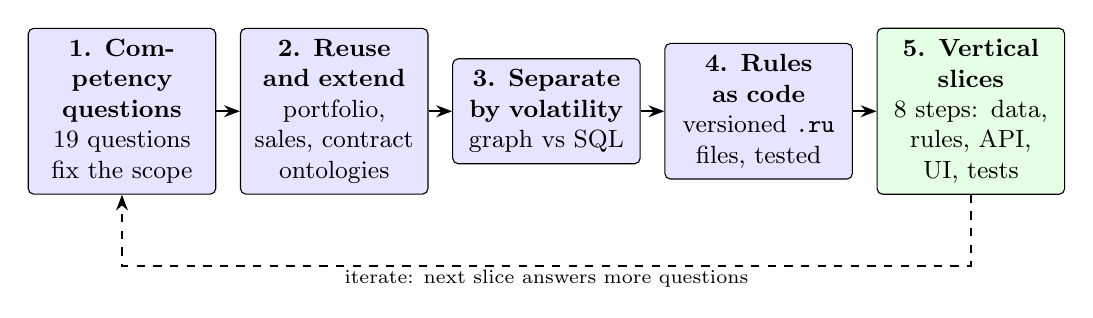
\begin{tikzpicture}[node distance=3mm,every node/.style={font=\scriptsize}]
\node[kg,text width=2.1cm] (a) {\textbf{1. Competency questions}\\19 questions fix the scope};
\node[kg,text width=2.1cm,right=of a] (b) {\textbf{2. Reuse and extend}\\portfolio, sales, contract ontologies};
\node[kg,text width=2.1cm,right=of b] (c) {\textbf{3. Separate by volatility}\\graph vs SQL};
\node[kg,text width=2.1cm,right=of c] (d) {\textbf{4. Rules as code}\\versioned \texttt{.ru} files, tested};
\node[app,text width=2.1cm,right=of d] (e) {\textbf{5. Vertical slices}\\8 steps: data, rules, API, UI, tests};
\foreach \x/\y in {a/b,b/c,c/d,d/e}{\draw[arr] (\x)--(\y);}
\draw[arr,dashed] (e.south)--++(0,-9mm)-|(a.south) node[lbl,pos=.25,below]{iterate: next slice answers more questions};
\end{tikzpicture}
\end{frame}

\begin{frame}{Methodology: separate by volatility}
\centering
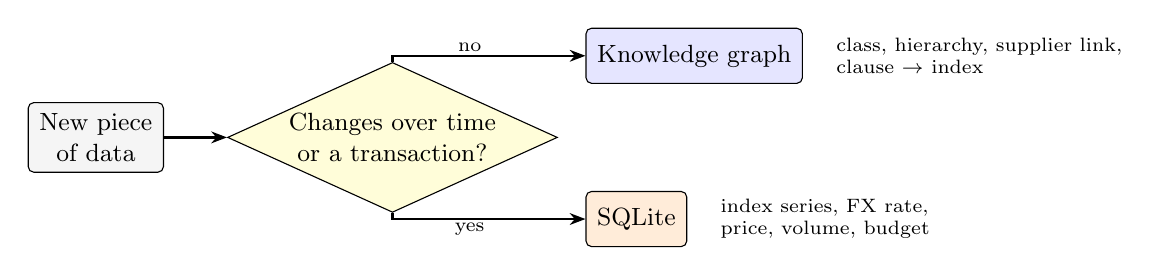
\begin{tikzpicture}[node distance=8mm]
\node[box] (q) {New piece\\of data};
\node[diamond,draw,aspect=2.2,fill=yellow!15,font=\small,align=center,right=of q,inner sep=1pt] (d) {Changes over time\\or a transaction?};
\node[kg,above right=2mm and 14mm of d] (g) {Knowledge graph};
\node[db,below right=2mm and 14mm of d] (s) {SQLite};
\draw[arr] (q)--(d);
\draw[arr] (d)|-node[lbl,pos=.7,above]{no}(g);
\draw[arr] (d)|-node[lbl,pos=.7,below]{yes}(s);
\node[font=\scriptsize,align=left,right=3mm of g] {class, hierarchy, supplier link,\\clause $\to$ index};
\node[font=\scriptsize,align=left,right=3mm of s] {index series, FX rate,\\price, volume, budget};
\end{tikzpicture}
\end{frame}

\begin{frame}{Methodology: rules as code}
\centering
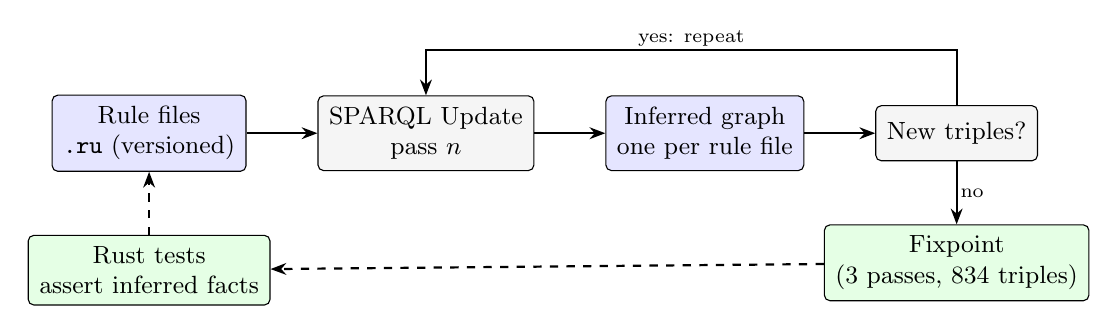
\begin{tikzpicture}[node distance=9mm]
\node[kg] (ru) {Rule files\\\texttt{.ru} (versioned)};
\node[box,right=of ru] (up) {SPARQL Update\\pass $n$};
\node[kg,right=of up] (inf) {Inferred graph\\one per rule file};
\node[box,right=of inf] (chk) {New triples?};
\node[app,below=8mm of chk] (done) {Fixpoint\\(3 passes, 834 triples)};
\node[app,below=8mm of ru] (test) {Rust tests\\assert inferred facts};
\draw[arr] (ru)--(up);\draw[arr] (up)--(inf);\draw[arr] (inf)--(chk);
\draw[arr] (chk)--node[lbl,right]{no}(done);
\draw[arr] (chk.north)--++(0,7mm)-|(up.north) node[lbl,pos=.25,above]{yes: repeat};
\draw[arr,dashed] (test)--(ru);
\draw[arr,dashed] (done)--(test);
\end{tikzpicture}
\end{frame}

\begin{frame}{Methodology: vertical slices}
\centering
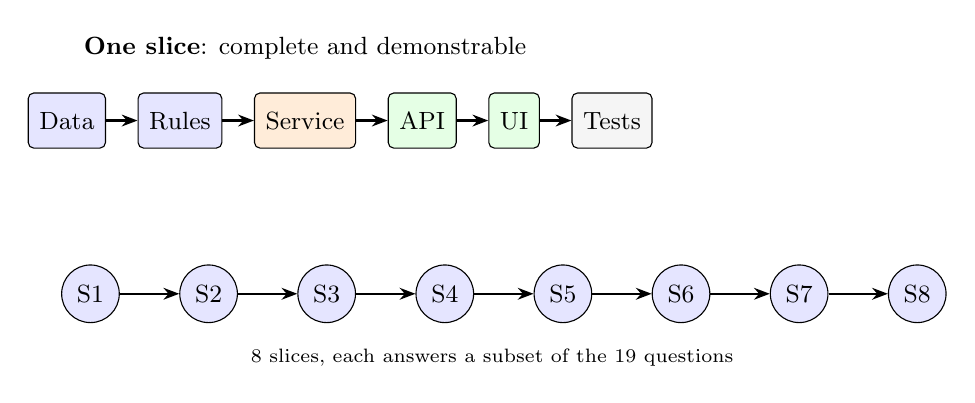
\begin{tikzpicture}[node distance=4mm]
\node[kg] (d1) {Data};
\node[kg,right=of d1] (r1) {Rules};
\node[db,right=of r1] (s1) {Service};
\node[app,right=of s1] (a1) {API};
\node[app,right=of a1] (u1) {UI};
\node[box,right=of u1] (t1) {Tests};
\foreach \x/\y in {d1/r1,r1/s1,s1/a1,a1/u1,u1/t1}{\draw[arr] (\x)--(\y);}
\node[font=\small,above=3mm of s1] {\textbf{One slice}: complete and demonstrable};
\foreach \i in {1,...,8}{
  \node[circle,draw,fill=blue!10,minimum size=7mm,font=\small] (c\i) at ({1.5*\i-1.2},-2.2) {S\i};
}
\foreach \i/\j in {1/2,2/3,3/4,4/5,5/6,6/7,7/8}{\draw[arr] (c\i)--(c\j);}
\node[font=\scriptsize,below=2mm of c4,xshift=6mm] {8 slices, each answers a subset of the 19 questions};
\end{tikzpicture}
\end{frame}

\begin{frame}{T-Box: the schema}
\begin{columns}[T]
\begin{column}{.55\textwidth}
\small
\begin{tabular}{@{}lrrr@{}}
\toprule
Module & Cls & OP & DP\\\midrule
VWGroup & 26 & 18 & 8\\
Sales & 16 & 22 & 15\\
Contracts & 12 & 10 & 11\\
Finance & 4 & 3 & 3\\
Supply & 3 & 6 & 4\\
Risk & 5 & 2 & 0\\
Market & 9 & 7 & 7\\
Campaign & 4 & 3 & 0\\\midrule
\textbf{Total} & \textbf{79} & \textbf{71} & \textbf{48}\\\bottomrule
\end{tabular}
\end{column}
\begin{column}{.42\textwidth}
\begin{itemize}\small
\item Hierarchy: Product $\supset$ Model $\supset$ Electric / Hybrid / Combustion (disjoint)
\item Defined classes via \texttt{equivalentClass}
\item Inverse and sub-property axioms
\item \texttt{IndexationClause}: weight, pass-through
\item Risk classes are \alert{derived}, never asserted
\end{itemize}
\end{column}
\end{columns}
\end{frame}

\begin{frame}{T-Box: the exposure path}
\centering
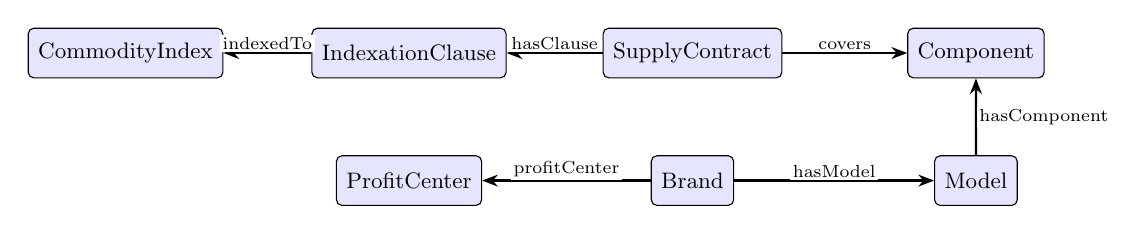
\begin{tikzpicture}[x=1cm,y=1cm,scale=.9,transform shape]
\node[kg] (idx) at (0,0) {CommodityIndex};
\node[kg] (cl) at (4,0) {IndexationClause};
\node[kg] (ct) at (8,0) {SupplyContract};
\node[kg] (co) at (12,0) {Component};
\node[kg] (md) at (12,-1.8) {Model};
\node[kg] (br) at (8,-1.8) {Brand};
\node[kg] (pc) at (4,-1.8) {ProfitCenter};
\draw[arr] (cl)--node[lbl,above]{indexedTo}(idx);
\draw[arr] (ct)--node[lbl,above]{hasClause}(cl);
\draw[arr] (ct)--node[lbl,above]{covers}(co);
\draw[arr] (md)--node[lbl,right]{hasComponent}(co);
\draw[arr] (br)--node[lbl,above]{hasModel}(md);
\draw[arr] (br)--node[lbl,above]{profitCenter}(pc);
\end{tikzpicture}
\end{frame}

\begin{frame}[fragile]{A-Box: the instances}
\begin{itemize}\small
\item 1,695 asserted triples: group, brands, models, 24 contracts, clients, markets, campaigns
\item Supply A-Box \alert{generated} by \texttt{tools/gen\_supply\_abox.py}
\item SQLite facts written into \texttt{graph/erp-facts} (165 triples) at load
\end{itemize}
{\footnotesize
\begin{verbatim}
vw:Clause_22_NaturalRubber a vw:IndexationClause ;
  vw:indexedTo vw:Index_NaturalRubber ;
  vw:indexWeight "0.40"^^xsd:decimal ;
  vw:passThroughRatio "1.00"^^xsd:decimal .
\end{verbatim}}
\end{frame}

\begin{frame}{Triples after load}
\centering
\begin{tabular}{lr}
\toprule Role & Triples\\\midrule
T-Box (8 files) & 591\\
A-Box (7 files) & 1,695\\
Original SWRL rules (documentation) & 547\\
ERP facts from SQLite & 165\\
Inferred by rules & 834\\\midrule
\textbf{Total} & \textbf{3,832}\\\bottomrule
\end{tabular}
\end{frame}

\begin{frame}[fragile]{Reasoning without a reasoner}
\begin{itemize}\small
\item No OWL/SWRL reasoner: JVM too heavy for a tiny VPS
\item SWRL rules ported to \alert{SPARQL Update}, applied to a \alert{fixpoint} (3 passes)
\item Each rule file $\to$ own graph: every inferred edge has provenance
\end{itemize}
{\footnotesize
\begin{verbatim}
INSERT { GRAPH <.../inferred> {
  ?model a vw:CommodityExposedModel ;
         vw:exposedToIndex ?index } }
WHERE { ?model vw:hasComponent ?c .
        ?contract vw:contractCoversComponent ?c ;
                  vw:exposedToIndex ?index }
\end{verbatim}}
\small Trade-off: lose open-world consistency checking; gain small footprint and testable rules.
\end{frame}

\begin{frame}{Architecture and infrastructure}
\centering
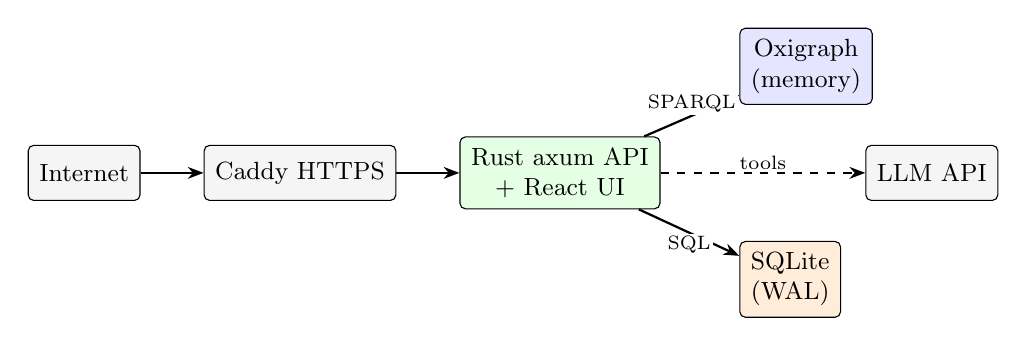
\begin{tikzpicture}[node distance=4mm]
\node[box] (net) {Internet};
\node[box,right=8mm of net] (cad) {Caddy HTTPS};
\node[app,right=8mm of cad] (api) {Rust axum API\\+ React UI};
\node[kg,above right=4mm and 10mm of api] (kgs) {Oxigraph\\(memory)};
\node[db,below right=4mm and 10mm of api] (sql) {SQLite\\(WAL)};
\node[box,right=26mm of api] (llm) {LLM API};
\draw[arr](net)--(cad);\draw[arr](cad)--(api);
\draw[arr](api)--node[lbl,above]{SPARQL}(kgs);
\draw[arr](api)--node[lbl,below]{SQL}(sql);
\draw[arr,dashed](api)--node[lbl,above]{tools}(llm);
\end{tikzpicture}
\begin{itemize}\small
\item Oxigraph: ${\sim}$15 ms load, $<$9 MB RAM; GraphDB needs ${\sim}$3 GB
\item Docker multi-stage build; \texttt{make deploy}; CI tests, deploy on merge
\end{itemize}
\end{frame}

\begin{frame}{Hybrid query flow}
\centering
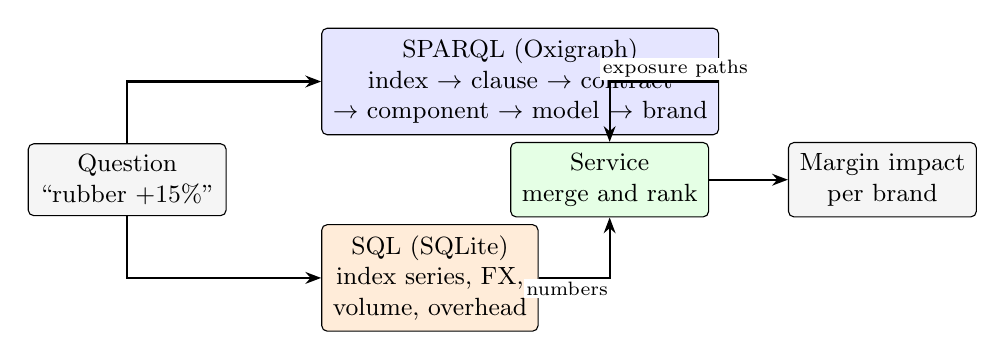
\begin{tikzpicture}[node distance=8mm]
\node[box] (q) {Question\\``rubber +15\%''};
\node[kg,above right=1mm and 12mm of q] (sp) {SPARQL (Oxigraph)\\index $\to$ clause $\to$ contract\\$\to$ component $\to$ model $\to$ brand};
\node[db,below right=1mm and 12mm of q] (sq) {SQL (SQLite)\\index series, FX,\\volume, overhead};
\node[app,right=36mm of q] (mg) {Service\\merge and rank};
\node[box,right=10mm of mg] (out) {Margin impact\\per brand};
\draw[arr] (q)|-(sp);\draw[arr] (q)|-(sq);
\draw[arr] (sp)-|node[lbl,pos=.2,above]{exposure paths}(mg);
\draw[arr] (sq)-|node[lbl,pos=.2,below]{numbers}(mg);
\draw[arr] (mg)--(out);
\end{tikzpicture}
\end{frame}

\begin{frame}{Hybrid query: ``rubber +15\%''}
\begin{enumerate}
\item SPARQL walks index $\to$ clause $\to$ contract $\to$ component $\to$ model $\to$ brand
\item SQL supplies index series, FX, volume, overhead
\item Service merges and ranks
\end{enumerate}
\[
P(t)=P_0\Bigl(1+\sum_i w_i\,\rho_i\Bigl(\tfrac{I_i(t)}{I_i(0)}-1\Bigr)\Bigr)\cdot f(t)
\]
\small Contract 22: rubber $w{=}0.40,\ \rho{=}1$ $\Rightarrow$ +15\% rubber = +6\% tyre price.
\end{frame}

\begin{frame}{19 questions, 5 domains}
\small
\begin{tabular}{@{}ll@{}}
\toprule
Finance & commodity/FX shock, margin floor, FX spend, discount tiers\\
Procurement & supplier failure, single-sourced, expiring, lead time\\
Strategy & subsidy, CO$_2$ target, rival price cut, site, powertrain mix\\
Sales & hot leads, campaigns vs capacity, lease vs loan\\
Scenario & combined ``bad year'', margin trace\\
\bottomrule
\end{tabular}
\vspace{3mm}

Each = service + UI view + chat tool + Rust test.
\end{frame}

\begin{frame}{Explain graph: example route}
\centering
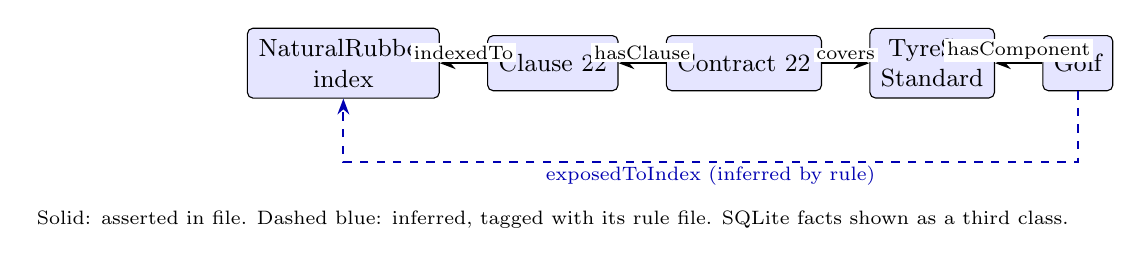
\begin{tikzpicture}[node distance=6mm,every node/.style={font=\scriptsize}]
\node[kg] (i) {NaturalRubber\\index};
\node[kg,right=of i] (c) {Clause 22};
\node[kg,right=of c] (k) {Contract 22};
\node[kg,right=of k] (p) {TyreSet\\Standard};
\node[kg,right=of p] (m) {Golf};
\draw[arr] (c)--node[lbl,above]{indexedTo}(i);
\draw[arr] (k)--node[lbl,above]{hasClause}(c);
\draw[arr] (k)--node[lbl,above]{covers}(p);
\draw[arr] (m)--node[lbl,above]{hasComponent}(p);
\draw[arr,dashed,blue!70!black] (m.south)--++(0,-9mm)-|node[lbl,pos=.25,below]{exposedToIndex (inferred by rule)}(i.south);
\node[below=14mm of c,font=\scriptsize] {Solid: asserted in file. Dashed blue: inferred, tagged with its rule file. SQLite facts shown as a third class.};
\end{tikzpicture}
\end{frame}

\begin{frame}{Explainability}
\begin{itemize}
\item \textbf{Explain graph}: shortest routes between two entities over allow-listed predicates
\item Edges classed: \textit{asserted} (file), \textit{inferred} (rule file), \textit{ERP fact} (SQLite)
\item Example: rubber $\to$ clause $\to$ Contract 22 $\to$ TyreSet\_Standard $\to$ Golf
\item \textbf{Chat}: LLM calls 21 tools; never sees SQL/SPARQL; key stays on server; streamed replies; rule-based fallback
\end{itemize}
\end{frame}

\begin{frame}{Evaluation and limitations}
\begin{columns}[T]
\begin{column}{.48\textwidth}
\textbf{Results}
\begin{itemize}\small
\item Rust tests: rules, services, chat, LLM stub, auth
\item Fixpoint: 3 passes, 3,832 triples
\item ${\sim}$11 MB memory serving
\end{itemize}
\end{column}
\begin{column}{.48\textwidth}
\textbf{Limits}
\begin{itemize}\small
\item Synthetic, calibrated data
\item No DL consistency checking
\item Penalty/renewal clauses not modelled
\end{itemize}
\end{column}
\end{columns}
\end{frame}

\begin{frame}{Conclusion}
\begin{itemize}
\item Structure in an ontology, numbers in SQL, joined by IRI
\item SPARQL fixpoint rules replace the reasoner
\item Every answer traceable back to graph facts
\item Next: budget-vs-actual page, HTTP tests, LLM quality evaluation
\end{itemize}
\vfill\centering\Large Questions?
\end{frame}

\end{document}
